\documentclass{article}

\usepackage[francais]{babel}
\def\printlandscape{\special{landscape}}    % Works with dvips.
%\usepackage{pstricks,pst-node,pst-tree}
%\usepackage{amssymb}
\usepackage[utf8]{inputenc}
\usepackage[T1]{fontenc} 
\usepackage{fancybox} % for shadow and Bitemize
\usepackage{alltt}
\usepackage{graphicx}
\usepackage{caption} 

%\usepackage{epsfig}
\usepackage{fullpage}
%\usepackage{fancyhdr}
%\usepackage{moreverb}
%\usepackage{xspace}
\usepackage[colorlinks,hyperindex,bookmarks,linkcolor=blue,citecolor=blue,urlcolor=blue]{hyperref}
\usepackage{array,multirow,makecell}
\setcellgapes{1pt}
\makegapedcells
\newcolumntype{R}[1]{>{\raggedleft\arraybackslash }b{#1}}
\newcolumntype{L}[1]{>{\raggedright\arraybackslash }b{#1}}
\newcolumntype{C}[1]{>{\centering\arraybackslash }b{#1}}
\usepackage{wrapfig}
\usepackage{epsf}

\title{Rapport de Projet GMIN332 :\\ Gestion de données complexes}

\author{Par : ALIJATE Mehdi - COUSOT Kevin - NEGROS Hadrien}

\date{15 Janvier 2014}

         
\begin{document}

\maketitle
\tableofcontents

\begin{abstract}
Accès et consultation de données provenant de différentes solutions de persistance (gros volumes de données distribuées et hétérogènes) au travers d'un démonstrateur.
\end{abstract}








\newpage 
%-----------------------------------------------------------
\section{Introduction}\label{sec:intro}
Les systèmes NoSQL et les technologies du Web Sémantique sont une altérnative aux SGBD classiques. Cependant, elles sont encore très loin d'être couramment utilisées, comme celles du monde relationnel "classique". \\
Néanmoins, de grands acteurs d'internet (\textit{comme Facebook (Cassandra Project puis HBase), Google (BigTable), Ubuntu One (CouchDB)... etc.}) commencent à exploiter des bases de données de type NoSQL. L'avantage de celà, c'est que la majorité de ces projets est open source et sous licence libre.
\\
Dans notre projet, nous avons voulu explorer les différentes technologies qui puissent gérer des données RDF. Nous avons donc étudié un système basé sur le triple store (\textbf{TDB}), mais aussi une solution basée sur le mapping de bases relationnelles (\textbf{D2RQ}), ou bien encore une solution basée sur des bases NoSQL, avec des bases orientées "graphes" (\textbf{Hbase et Neo4j}).
\\
Le but de ce projet est d’exploiter différentes sources de données, gérées au travers de plusieurs systèmes de gestion de données, afin de permettre un accès et consultation de ces derniers. Ceci, via une application permettant d'interconnecter ces sources de données, basée sur l'API de Jena.





%-----------------------------------------------------------

\section{Jeu de données}
/\textbf{TODOO à finir}\\
\subsection{Description}
Le jeu de données utilisé représente des données de vocabulaire de l'\textbf{INSEE} et des données\textbf{ Geonames}.
L’INSEE (Institut National de la Statistique et des Etudes Economiques) collecte, produit, analyse et diffuse des informations sur l'économie et la société françaises. A ce titre, il conduit des recensements et des enquêtes, il gère des bases de données et exploite aussi des sources administratives.
Geonames est une base de données géographique gratuite et librement accessible sur Internet (www.geonames.org). La base regroupe plus de 8 millions de noms de lieux géographiques, et beaucoup d’informations autours de ces lieux (par exemple la  population, la subdivision administrative, le code postal, la latitude, la longitude, l'altitude, etc.). 
\\
\subsection{Schéma}


\textbf{//A finir avec une description plus précise de chaque données avec un schéma d'interconnexion
}

\section{Analyse du système}

\subsection{API de Jena}
Jena est une API Java qui peut être utilisée pour créer et manipuler des données RDF . Jena possède des classes pour représenter des graphes, des ressources, des propriétés et des littéraux.

Ce projet est uni autour de l'API de Jena (Cf. Section \ref{sec:Jena}) et de ses modèles.
\begin{center}
 

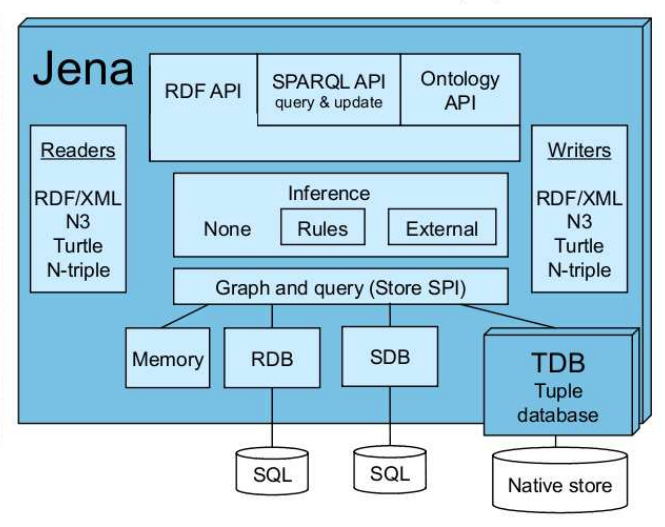
\includegraphics[scale=0.5]{archi_jena.jpeg} 
\captionof{figure}{Vue Générale de l'architecture JENA}
\label{fig_jena}
\end{center}
\begin{itemize}
\item \textbf{TDB :} c'est un triple store avec une solution souple sans schéma prédéfini. 
\item \textbf{D2RQ : } ce système est adapté au stockage des données de fichiers csv par exemple, dans une relation d'un schéma relationnel. Avec Direct Mapping, on peut facilement traduire un modèle relationnel en RDF.\\
\begin{center}
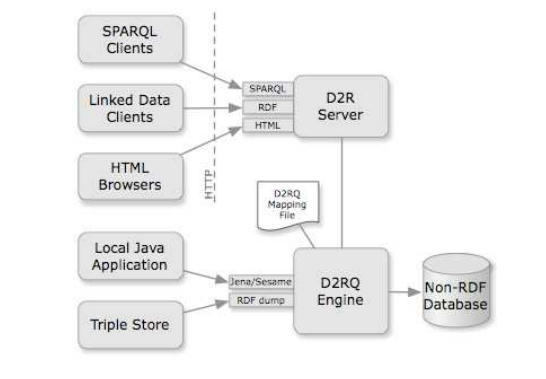
\includegraphics[scale=0.5]{archi_D2RQ.jpeg} 
\captionof{figure}{Vue Générale de l'architecture D2RQ}
\label{fig_d2rq}
\end{center}

\item \textbf{Neo4j :} est une base de données graphique, et il est un bon modèle de stockage de données pour une ontologie. Neo4j est robuste (entièrement ACID).



\item \textbf{HBase :} Jena-HBase fournit un stockage évolutif et une solution d'interrogation qui prend en charge toutes les fonctionnalités de la spécification RDF.


\end{itemize}



\subsection{Intérrogation SPARQL}
La réprésentation Model spécifique à Jena a permi l'union obtenus à partir de nos sources de données. Les requêtes SPARQL sont effectuées sur le modèle ainsi créé.\\
Chaque triple store définit ses propres fonctions à côté de celles de SPARQL (ARQ pour Jena). Pour gérer les requêtes SPARQL, Jena utilise sa propre librairie \textit{ARQ}. Cette librairie définit également sa propre syntaxe, compatible notre mode de requêtage SPARQL, cela y ajoute des fonctionnalités semblables à ce qu'on peut trouver dans MySql par exemple, comme COUNT, MAX, etc, car ces fonctions ne sont pas gérées par défaut par SPARQL.



%-----------------------------------------------------------
\section{Réalisation}

\subsection{Triple store : TDB}
//TODO


%-----------------------------------------------------------

\subsection{D2RQ}

//TODO

%-----------------------------------------------------------
\subsection{Neo4j}
//TODO



%-----------------------------------------------------------



\subsection{HBase}
//TODO
%-----------------------------------------------------------

\subsection{Modèle JENA : Intégration}\label{sec:Jena}
//TODO

%-----------------------------------------------------------


\section{Démonstrateur}

\subsection{Principe}
//TODO

\subsection{Requêtes}

//TODO
%-----------------------------------------------------------


\section{Discussion et Conclusion }
//TODO
%-----------------------------------------------------------


\section{Sources}

//TODO

%-----------------------------------------------------------

\end{document}

%%% Local Variables:
%%% mode: latex
%%% TeX-master: t
%%% coding: utf-8
%%% End:
